\documentclass[deposito, acronym, symbols]{fei}

%\usepackage{glossaries}
\usepackage{subcaption} 
\usepackage{graphicx}
\usepackage{float}
%\usepackage{units}
\usepackage[portuguese]{algorithm2e}
\usepackage{biblatex}
\usepackage{amsmath}
\usepackage{listings}
\usepackage[utf8]{inputenc}
\usepackage{chngcntr} %Faz com que o numero das notas de rodape aumente crescentemente.
\usepackage{appendix}
\counterwithout{footnote}{chapter}% "
\usepackage{siunitx}
\sisetup{output-exponent-marker=\ensuremath{\mathrm{e}}} %Escrita que precede cada entrada na lista de ilustrações.
\renewcommand{\cftfigurepresnum}{Figura }
\setlength{\cftfigurenumwidth}{5.7em}

\usepackage{titling}

%\makeglossaries
%%\newacronym[] {achpt} {ACT} {Aparecido ChupeTão}

\newacronym[longplural=Associações Brasileiras de Normas Técnicas]{abnt}{ABNT}{Associação Brasileira de Normas Técnicas}

\newacronym{ibge}{IBGE}{Instituto Brasileiro de Geografia e Estatística}

\newacronym{ashrae}{ASHRAE}{\textit{American Society of Heating, Refrigerating and Air-Conditioning Engineers}}

\newacronym{nbr}{NBR}{Norma Brasileira}

\newacronym{pmv}{PMV}{\textit{Predicted Mean Vote}}
	
\newacronym{ppd}{PPD}{\textit{Predicted Percentage of Dissatisfied}}
		
\newacronym{vgd}{VGD}{Ventilação Geral Diluidor}
		
\newacronym{vgl}{VGL}{Ventilação Local Exaustora}
		
\newacronym{cfd}{CFD}{\textit{Computational Fluid Dynamics}}
		
\newacronym{pcb}{PCB}{\textit{Printed Circuit Board}}
		
\newacronym{sms}{SMS}{\textit{Short Message Service}}
		
%\newglossaryentry{pi}{parent=greek,type=symbols,name={\ensuremath{\pi}},sort=p,description={número irracional que representa [razão entre a circunferência de qualquer círculo e seu diâmetro]}}
		


\title{ESFORÇOS NA FURAÇÃO NO TORNO - Grupo C}
\author{ Felipe Estevão Coquito de Mello - 11.120.486-3 \\ Gabriel Mola da Silva - 11.120.255-2 \\ Netuno Trindade Torrente Rovaroto - 11.120.321-2 \\ Vitoria Fedatto Stefaneli - 11.120.497-0}
\cidade{São Bernardo do Campo}
\instituicao{Centro Universitário FEI}

\addbibresource{Referencias.bib}
%\bibliographystyle{plain}
\bibliography{Referencias}
\graphicspath{ {Imagens/}, {Tabelas/}}

\begin{document}
\maketitle

\begin{folhaderosto}
Relatório apresentado ao departamento de Engenharia Mecânica do Centro Universitário FEI, como parte dos requisitos de avaliação da disciplina ME140 – Usinagem. Solicitado pelo Prof. Adalto de Farias.
\end{folhaderosto}

\tableofcontents
\listoffigures
\listoftables

\begin{resumo}

A furação é um processo de usinagem muito utilizado na indústria, portanto, e como em todo processo de usinagem, é necessário saber como os esforços de usinagem afetam tal processo. Neste relatório será avaliado, por meio de ensaios, como os parâmetros velocidade de corte ($Vc$), avanço ($fn$) e o uso ou não de refrigeração, influenciam a furação no torno.Para título de comparação os dados foram analisados, também, no software Minitab e posteriormente gerados gráficos comparativos para cada parâmetro de corte e sua influência nos esforços de furação. Levando em consideração algumas falhas ou imprecisões durante a prática dos ensaios, os resultados obtidos foram satisfatórios com a teoria, e que o avanço é a variável que mais influencia e impacta ambos os esforços estudados.

\palavraschave{Usinagem. Esforços na furação. Otimização.}

\end{resumo}

\chapter{Introdução}

A furação é um processo de usinagem muito utilizada na indústria, portanto, e como em todo processo de usinagem, é necessário saber como os esforços de usinagem afetam tal processo. Contudo, o processo de furação ainda é muito pouco avançado em comparação com outros processos de usinagem como o fresamento e o torneamento.



\section{Problemas e motivações para o estudo}

No meio da confecções de peças, existe um enorme interesse na otimização dos processos, ou seja encontrar o melhor custo beneficio na produção de cada peça, porém sem comprometer o produto final para o cliente.

Neste contexto, se faz necessário o estudo de quais variáveis durante a furação da peça influencia diretamente na qualidade final do produto e quais variáveis otimizam a fabricação da peça final.


\section{Objetivos do trabalho}

O objetivo desse trabalho é estudar a influencia da velocidade de corte ($Vc$), do avanço ($f_n$)  e da refrigeração nos esforços de furação, utilizando uma maquina CNC. E com o auxílio do Minitab, gerar gráficos e um modelo empírico para o momento torsor em função dos parâmetros de corte e comparar com os resultados teóricos.

\chapter{Referencial teórico}

O processo de furação é um dos mais utilizados na indústria de manufatura e somente em alguns poucos casos os furos já vêm prontos (peças fundidas, forjadas, etc.). Isso torna o estudo de otimização da furação muito importante. (\textcite{diniz2002tecmat}).

Processos de usinagem que utilizam outras ferramentas como o torneamento e o fresamento evoluíram bastante com o tempo, porém na furação a ferramenta mais utilizada ainda é a broca helicoidal o que gera um atraso na evolução deste processo. Este atraso está relacionado com alguns fatores, mas o principal deles é que a broca helicoidal de aço rápido para ser utilizada com velocidades equivalentes ao de metal duro ($V_c$ = 200 $m/min$) necessita de uma rotação altíssima impossível de alcançar em um torno de furação comum. Mas com os tornos CNC sendo mais comumente utilizados no processo de furação é possível a cada dia ver uma evolução neste processo.  

\section{Características da broca helicoidal}

As brocas helicoidais são formadas por diversas partes, como mostra a Figura \ref{fig:broca}.

\begin{figure}[!htp]
    \centering
    \caption{Componentes da broca helicoidal}
    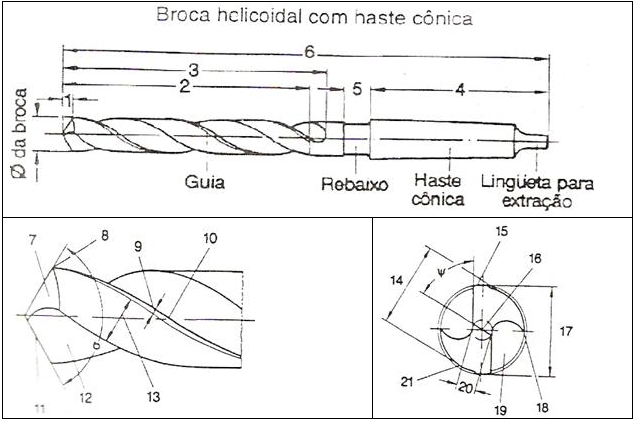
\includegraphics[width=0.7\linewidth]{Imagens/broca helicoidal.png}
    \smallcaption{Fonte: Adaptado de \textcite{diniz2002tecmat}}
    \label{fig:broca}
\end{figure}

Portanto, é importante saber algumas partes e sua funcionalidade, como por exemplo: a haste é a parte que fica presa à máquina, podendo ser cônica ou cilíndrica; corpo é o comprimento útil da broca, no casa da broca helicoidal o corpo tem dois canais em forma de hélice; a ponta é a parte cortante, com um ângulo que depende do material, e que deve ser afiada; as guias são suficientemente finas para que o atrito entre a broca e o material seja diminuído. Além disso, elas também possibilitam a entrada do fluido de refrigeração.


\section{Esforços de corte na furação}

Segundo \textcite{diniz2002tecmat} é necessário verificar as resistências das brocas à furação, sendo elas:
\begin{enumerate}
    \item resistência nas duas arestas de corte principais, devido ao corte do material;
    \item resistência de corte e de esmagamento da aresta transversal de corte;
    \item resistência ao atrito das guias com a parede do material e entre a superfície de saída da broca com o cavaco.
\end{enumerate}

Uma broca helicoidal é basicamente submetida somente à torção e à compressão quando em operação. Então para quantizar os esforços envolvidos no processo é preciso calcular o momento torsor ($M_t$) e a força de avanço ($F_f$) do processo. 

Para a broca fazer seu trabalho ela tem que vencer as três resistências citadas acima. Sendo assim, tem-se as equações \ref{eq Mtotal} e \ref{eq F_total}.

\begin{equation}
    \label{eq Mtotal}
    M_{total}= M_{ta}+M_{tb}+M_{tc}
\end{equation}

\begin{equation}
    \label{eq F_total}
    F_{total}= F_{fa}+F_{fb}+F_{fc}
\end{equation}

Onde $M_{total}$ e $F_{total}$ são, respectivamente, o momento torsor total e a força de avanço total, e os índices $a$, $b$ e $c$ são as contribuições das resistências nos esforços $M_{total}$ e $F_{total}$.

Para furação, o centro da broca ($D=0$) não haverá nem força, nem velocidade de corte e as máximas dessas grandezas acontecerão nas arestas laterais da broca. A Figura \ref{fig:vc sandvik} e a equação \ref{eq VC} mostram o detalhamento da $V_c$. 

\begin{figure}[!htp]
    \centering
    \caption{Velocidade de corte na broca helicoidal}
    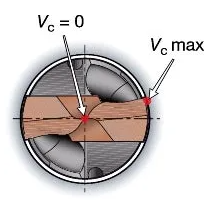
\includegraphics[width=0.3\linewidth]{Imagens/vc sandivik certo.png}
    \smallcaption{Fonte: Sandvik Coromant}
    \label{fig:vc sandvik}
\end{figure}

\begin{equation}
    \label{eq VC}
    V_c=\frac{{n}\times {\pi} \times{D}}{1000}
\end{equation}

Onde $D$ é o diâmetro da broca e $n$ a rotação da máquina.

Visto que existe uma velocidade de corte, nas brocas helicoidais também existe uma força de corte ($F_c$), que é a força necessária para a remoção do material da peça. Dito isto, é possível estimar a equação \ref{eq FC} para furo em cheio e broca normal com duas arestas de corte, segundo Kienzle. 

\begin{equation}
    \label{eq FC}
    F_c=\frac{K_{s1}\times{(\frac{D}{2})}}{\sin{\frac{\phi}{2}}}\times[{\frac{fn}{2}}\times{\sin{\frac{\phi}{2}}}]^{1-z}
\end{equation}

E para furação com um pré furo existente, tem-se a equação \ref{eq FCpf}.

\begin{equation}
    \label{eq FCpf}
    F_c=\frac{K_{s1}\times{(\frac{D-d_0}{2}})}{\sin{\frac{\phi}{2}}}\times[{\frac{fn}{2}}\times{\sin{\frac{\phi}{2}}}]^{1-z}
\end{equation}

Onde:

$K_{s1}$ é a pressão específica de corte;

$D$ é o diâmetro da broca;

$d_0$ é o diâmetro do pré furo;

$\phi$ é o ângulo de ponta da broca;

$z$ é o coeficiente de correção experimental.




Segundo os autores, o momento torsor se divide em: de 77\%-90\% devido às arestas principais, de 3\%-10\% devido à aresta transversal e, por fim, de 5\%-20\% devido ao atrito. 
E com a equação da $F_c$ definida, é possível estimar a equação \ref{eq Mt} em função da força de corte.

\begin{equation}
    \label{eq Mt}
    M_t=F_c\times{\frac{D+D_0}{2}}
\end{equation}

O $M_t$, segundo Kienzle, está descrito na equação \ref{eq MtKienzle}. Esta equação é válida tanto para furo em cheio ($d_0$=0), quanto para furação com pré furo.

\begin{equation}
    \label{eq MtKienzle}
    M_t=2\times{K_{s1corri}}\times{(\frac{D^2-d_0^2}{8})}\times{(\frac{fn}{2}})^{1-z}\times({\sin{\frac{\phi}{2}}})^{-z}
\end{equation}

O $K_{s1corri}$ é definido pela equação \ref{eq Ks1Kienzle}

\begin{equation}
    \label{eq Ks1Kienzle}
    K_{s1corri}=K_{s1tab}\times{(1+\frac{\gamma_{tab}-\gamma_{ef}}{100})}\times{\frac{HB_{mat}}{HB_{tab}}}\times{CL}
\end{equation}

Sendo:

$K_{s1tab}$: pressão específica tabelada para cada tipo de material;

$\gamma_{tab}$: ângulo de saída tabelado;

$\gamma_{ef}$: ângulo de saída efetivo;

$HB_{mat}$: dureza do material;

$HB_{tab}$: dureza do material tabelada;

$CL$: fator de correção para óleo de corte utilizado.

Além de Kienzle outros pesquisadores também fizeram equações para descrever o $M_t$ como Kronenberg, com a expressão \ref{eq Mtkr} e H. Daar, com a expressão \ref{eq Mthd}.

\begin{equation}
    \label{eq Mtkr}
    M_t=C_1\times{D}^{x1}\times{fn}^{y1}\times{CL}
\end{equation}

\begin{equation}
    \label{eq Mthd}
    M_t=C_3\times{D}^{2-x3}\times{fn}^{1-z3}\times{(D^{x3}-d_0^{x3})}\times{CL}
\end{equation}

$C_1$, $x1$, $y1$, $C_3$, $z3$ e $x3$ são constantes experimentais definidas pelos criadores das expressões acima. Enquanto que $D$ é o diâmetro da broca, $d_0$ é o diâmetro do pré furo, $fn$ é o avanço e $CL$ é o fator de correção do óleo.

Por fim, segundo \textcite{diniz2002tecmat} a força de avanço atua nas arestas principais (39\%-59\%), na aresta transversal (40\%-58\%) e também tem uma pequena influência no atrito (2\%-5\%). Para tanto, Kienzle e H. Daar propuseram fórmulas para a $F_f$ com pré-furo, demostradas nas equações \ref{eq FfKienzle} e \ref{eq ffhd}. E H. Daar, também propôs uma equação da força de avanço para furação em cheio, vista na equação \ref{eq FFhdc}

\begin{equation}
    \label{eq FfKienzle}
    F_{f}=0,4\times{K_{s1corri}}\times{({D^2-d_0^2})}\times{(\frac{fn}{2}})^{1-z}\times({\sin{\frac{\phi}{2}}})^{-z}
\end{equation}

\begin{equation}
    \label{eq ffhd}
    F_f=C_4\times{D}^{1-x4}\times{fn}^{1-y4}\times{(D^{x4}-d_0^{x4})}\times{CL}
\end{equation}


\begin{equation}
    \label{eq FFhdc}
    F_f=C_2\times{D}^{x2}\times{fn}^{y2}\times{CL}
\end{equation}

Sendo, $C_2$, $C_4$, $x2$, $x4$, $y2$ e $y4$, contantes empíricas das equações.



\chapter{Metodologia}

Em aula o orientado disponibilizou os dados, para iniciar o planejamento dos ensaios, os dados estão disponível na Tabela \ref{tab:Variaveis}.

\begin{table}[!htb]
 \centering
    \caption{Valores designados ao grupo}
    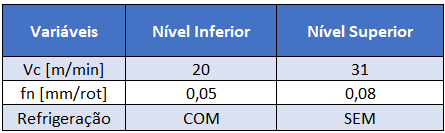
\includegraphics[width=0.7\linewidth]{Imagens/Exp04_variaveis.png}
    \smallcaption{Fonte: Autor}
    \label{tab:Variaveis}
 \end{table}

O planejamento dos ensaios foi executado utilizando o software Minitab, sendo composto de um Planejamento Fatorial Completo, com três fatores ($V_c$, $f_n$ e $Refigeralção$) sem réplica, em dois níveis, com um ponto central por bloco. O resultado deste planejamento está disponível na Tabela \ref{tab:Planejamento}.

\begin{table}[!htb]
 \centering
    \caption{Planejamento gerado com utilização do Minitab}
    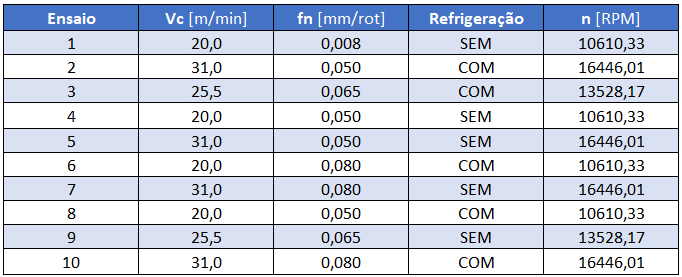
\includegraphics[width=0.9\linewidth]{Imagens/Exp04_planejamento.png}
    \smallcaption{Fonte: Autor}
    \label{tab:Planejamento}
 \end{table}

 \section{Experimento}

 O experimento foi realizado no Centro de Laboratórios Mecânicos da FEI (CLM), utilizando o Torno ROMI Centur 30D, visto na Figura \ref{fig:CNC}. E a ferramenta foi uma broca com ø6 $mm$, mostrada na Figura \ref{fig:Ferramenta} e o material de estudado foi o aço ABNT 1045.

\begin{figure}[!htp]
  \centering
  \begin{minipage}{0.4\textwidth}
    \centering
    \caption{Torno ROMI Centur 30D}
    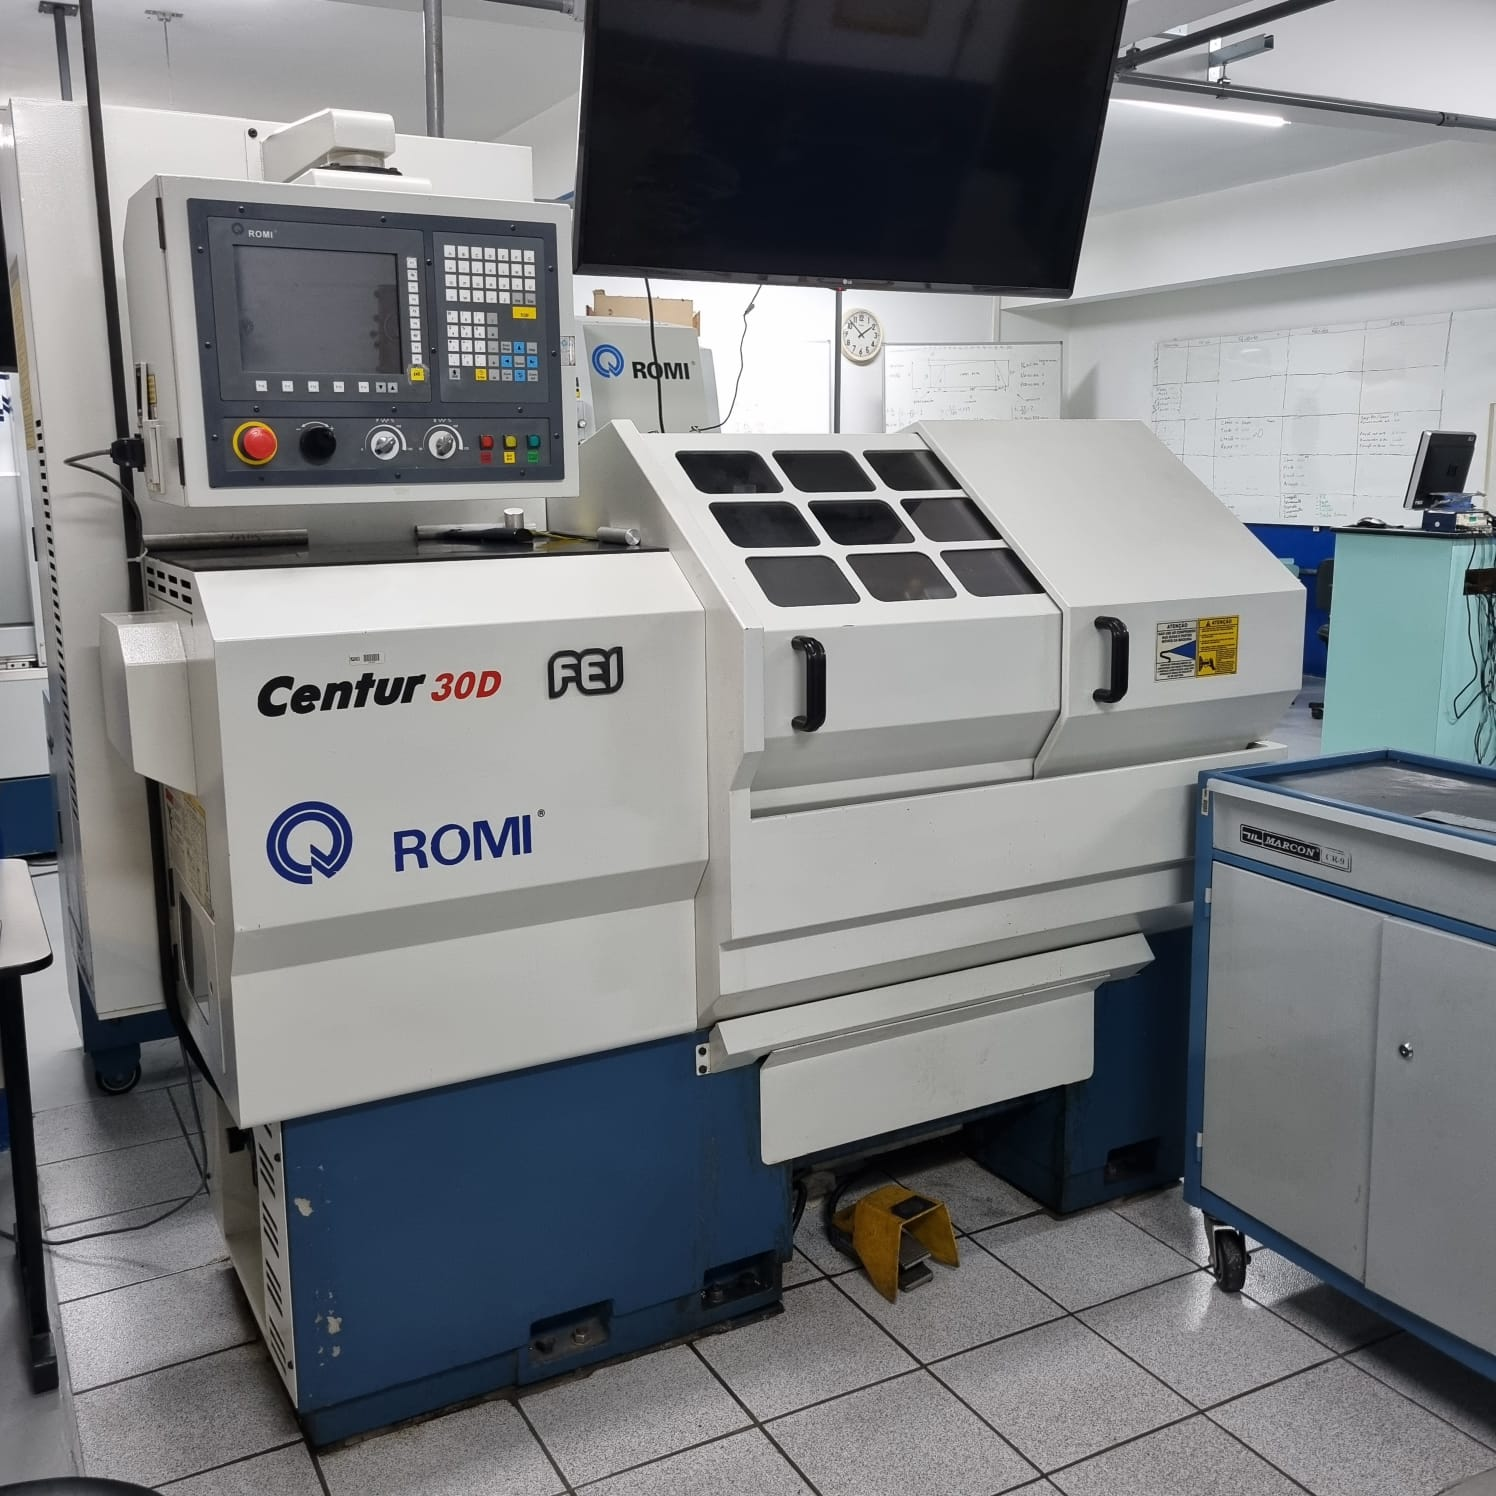
\includegraphics[width=1\linewidth]{Imagens/Exp04_torno.jpeg}
    \smallcaption{Fonte: Autor}
    \label{fig:CNC}
  \end{minipage}
  \hfill
  \begin{minipage}{0.4\textwidth}
        \caption{Ferramenta}
    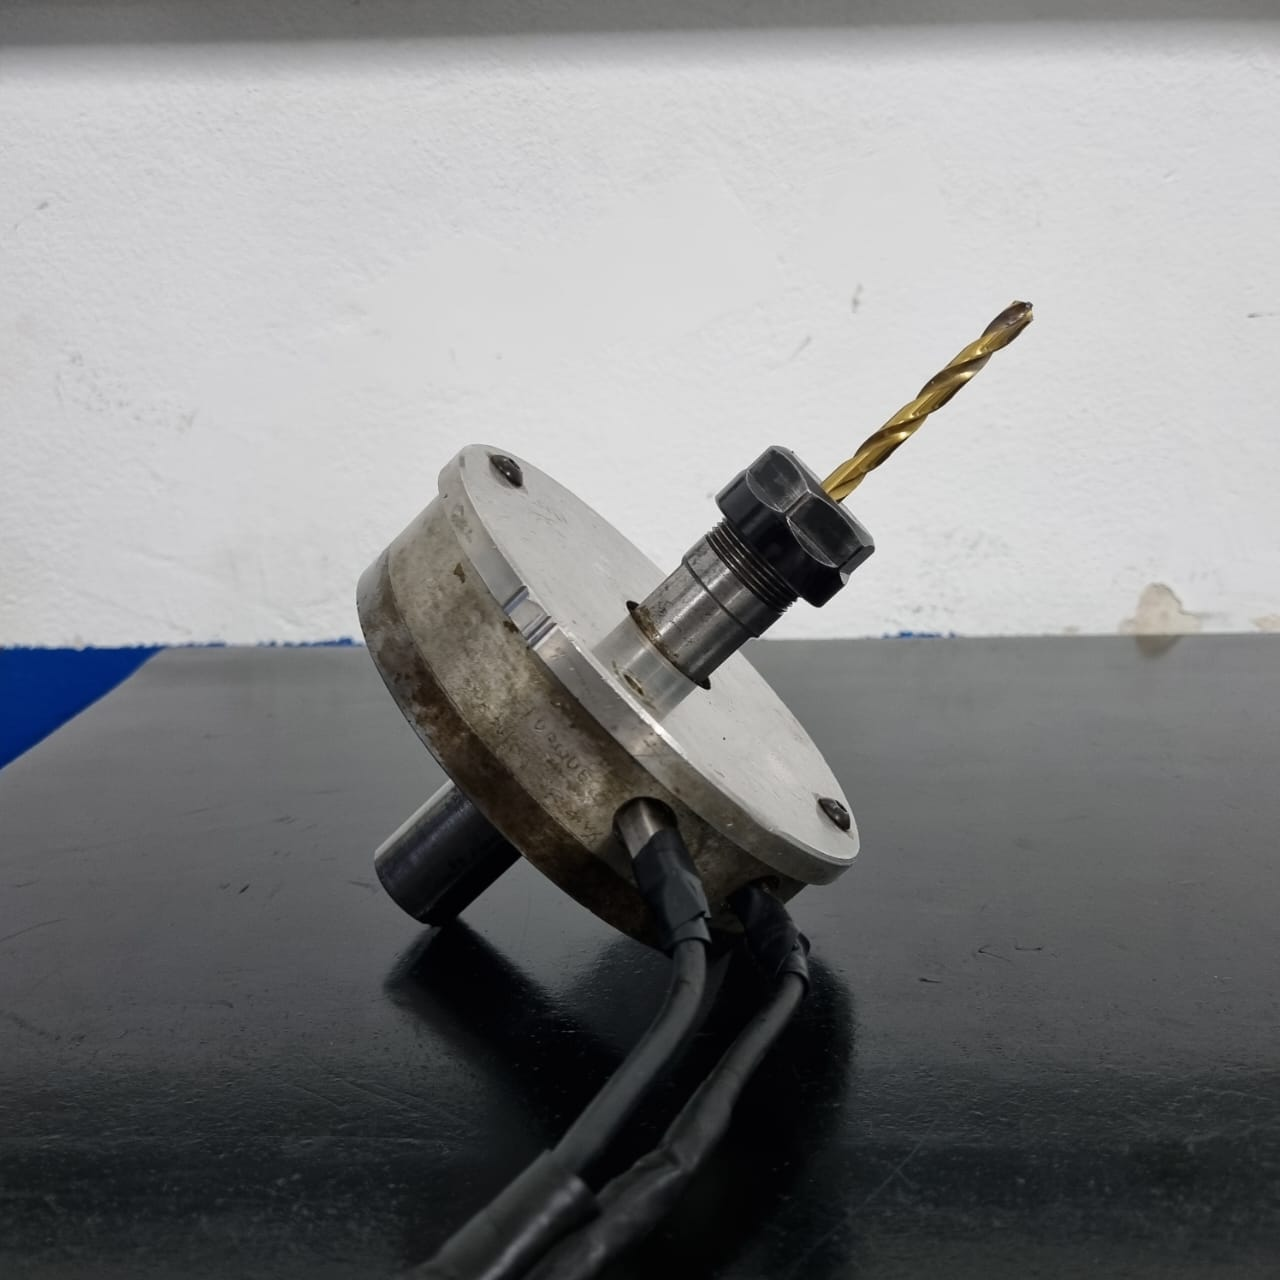
\includegraphics[width=1\linewidth]{Imagens/Exp04_ferramenta.jpeg}
    \smallcaption{Fonte: Autor}
    \label{fig:Ferramenta}
  \end{minipage}
\end{figure}

O experimento foi realizado com o objetivo de pegar os dados de esforços, através dos dados obtidos na medição dos Strain Gauge. Após a montagem da ferramenta e posicionamento da peça na placa de três castanhas, a sequência do experimento se deu por: 

\begin{enumerate}
    \item Atribui-se os valores correspondestes de $V_c$ e $f_n$ do ensaio a ser executado no torno a partir da folha de planejamento, assim como o uso ou não uso de refrigeração o qual será manipulado pelo técnico responsável;
    \item Iniciou-se, então, a operação de torneamento;
    \item Simultaneamente ao inicio da operação, iniciou a medição dos esforços no software do computador, indicado na Figura \ref{fig:comp};
    \item Finalizou-se a operação;
    \item Os dados do ensaio foram salvos;
    \item Repetiu-se o mesmo procedimento para os próximos ensaios.
\end{enumerate}

As Figuras \ref{fig:exp} e \ref{fig:blocos} e  mostram o interior do torno e os corpos de provas ao final do experimento, respectivamente.

\begin{figure}[!htp]
    \centering
    \caption{Interior do Torno}
    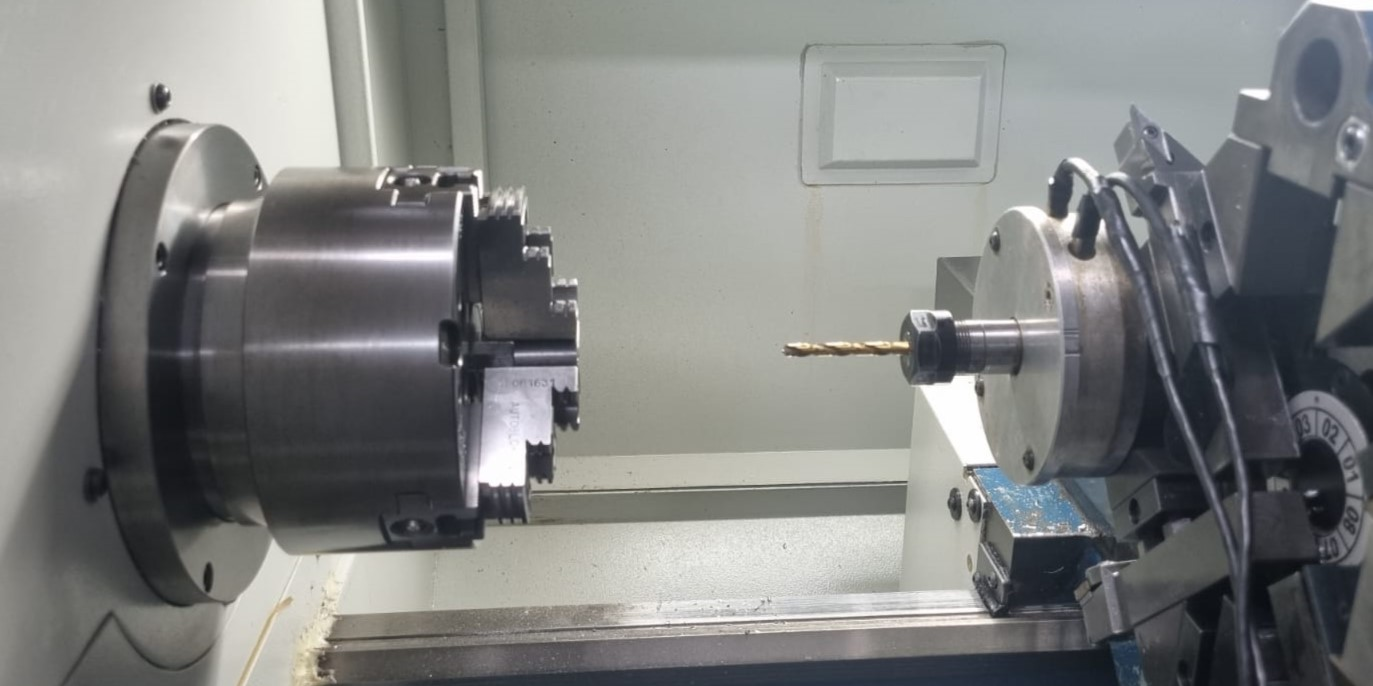
\includegraphics[width=0.8\linewidth]{Imagens/Exp04_interior.jpeg}
    \smallcaption{Fonte: Autor}
    \label{fig:exp}
\end{figure}


\begin{figure}[!htp]
  \centering
  \begin{minipage}{0.6\textwidth}
    \centering
    \caption{Computador com software de medição de esforços}
    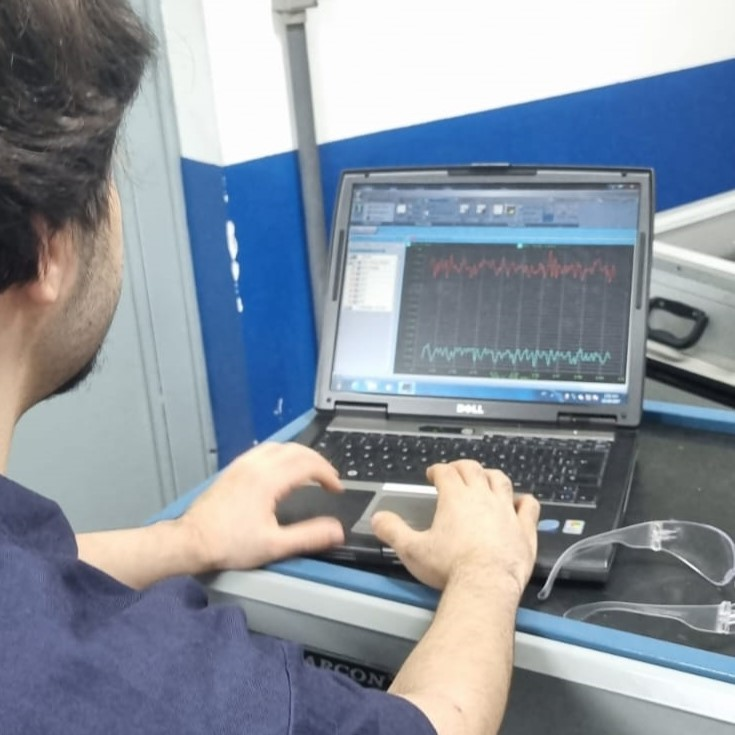
\includegraphics[width=1\linewidth]{Imagens/Exp04_computador.jpeg}
    \smallcaption{Fonte: Autor}
    \label{fig:comp}
  \end{minipage}
  \hfill
  \begin{minipage}{0.6\textwidth}
        \caption{Corpos de prova ao final do experimento}
    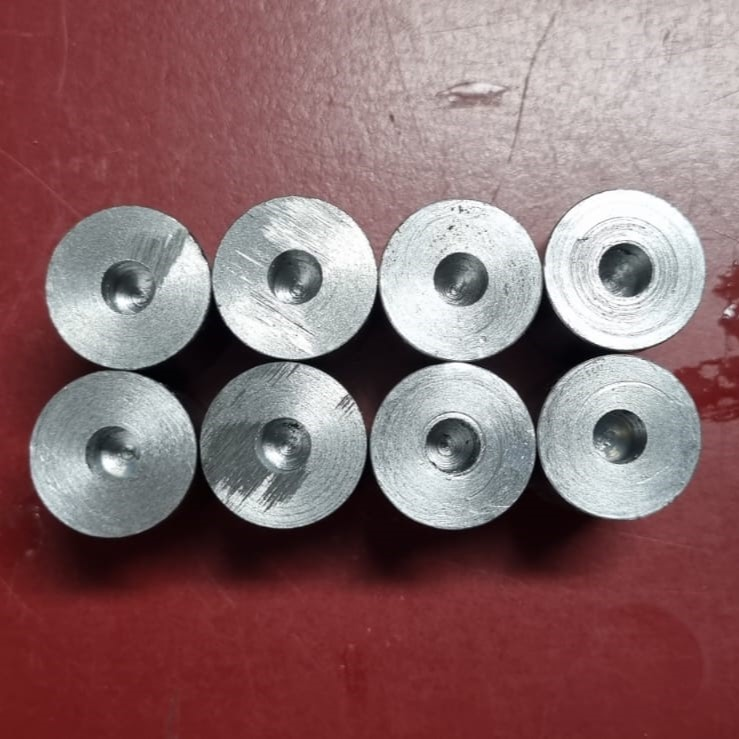
\includegraphics[width=1\linewidth]{Imagens/Exp04_blocos.jpeg}
    \smallcaption{Fonte: Autor}
    \label{fig:blocos}
  \end{minipage}
\end{figure}

\chapter{Resultados e Discussões}

Ao longo deste segmento, serão apresentados gráficos e tabelas gerados pelo Minitab, respaldando as constatações sobre quais parâmetros têm uma repercussão mais expressiva nos esforços enfrentados pela ferramenta. O principal objetivo é examinar de que maneira e com qual intensidade os parâmetros de corte (avanço (fn), velocidade de corte (Vc) e Refrigeração), influenciam nos seguintes esforços: Força de avanço (Fa) e Momento torsor (Mt).

\section{Entrada de Dados}

Inicialmente, os dados da Tabela \ref{tab:input} foram incorporados ao Minitab, permitindo que o software dispusesse das informações necessárias para efetuar as comparações desejadas. Esses dados foram obtidos a partir da experiência prática, utilizando células de carga. Adicionalmente, configuramos o Minitab de modo a proporcionar a análise mais apropriada para o nosso contexto, apresentando os resultados desejados correspondentes.

\begin{table}[!htb]
 \centering
    \caption{Planejamento gerado com utilização do Minitab}
    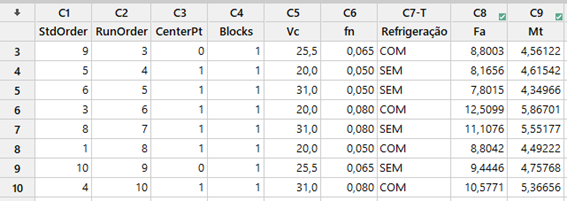
\includegraphics[width=0.8\linewidth]{Imagens/input furação.png}
    \smallcaption{Fonte: Autor}
    \label{tab:input}
 \end{table}

 \section{Regressão Fatorial} \label{regressao}

 Vamos iniciar nossa análise com a regressão fatorial, uma abordagem que nos permitirá estimar diversos resultados do experimento em questão.
 
 \subsection{Regressão Fatorial (Força de Avanço em função de fn, Vc, Refrigeração)} \label{regressaof}

A Tabela \ref{tab:var1} fornece uma variedade de informações valiosas, e ao examinar a coluna "Valor P", destaca-se que os valores associados ao avanço (fn) são os menores da tabela, sendo o único parâmetro dentre os três analisados (Fn, Vc e Refrigeração) abaixo de 0,05 (valor de alpha). Essa constatação aponta para uma confiança substancial, aproximadamente 95\%, indicando que o avanço (fn) exerce uma influência notável na força de avanço.

\begin{table}[!htb]
 \centering
    \caption{Análise de Variância (Fa)}
    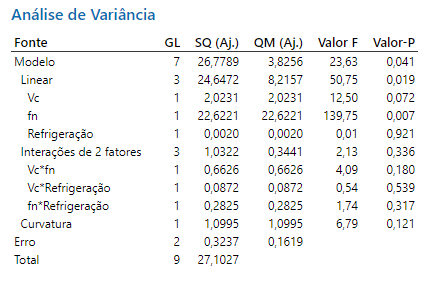
\includegraphics[width=0.8\linewidth]{Imagens/variancia 1.png}
    \smallcaption{Fonte: Autor}
    \label{tab:var1}
 \end{table}

Ao focar na mesma tabela, mas agora na coluna "Valor F", nota-se que o avanço (fn) apresenta o maior Valor F. Esse resultado sugere que a curva associada a esse parâmetro, a ser discutida nos próximos tópicos, terá uma inclinação considerável. Portanto, podemos inferir que o avanço desempenha um papel significativo no esforço analisado, ou seja, na força de avanço.

\begin{figure}[!htp]
    \centering
    \caption{Gráfico de Pareto dos Efeitos Padronizados (Fa)}
    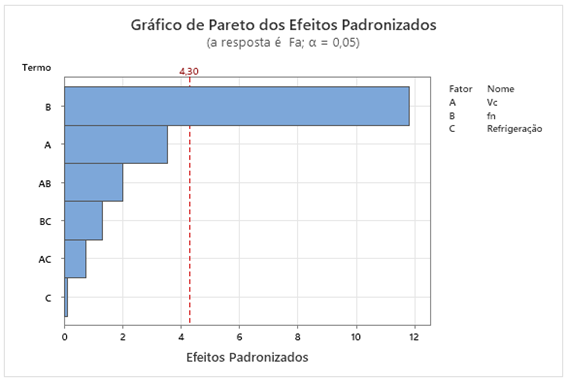
\includegraphics[width=0.8\linewidth]{Imagens/pareto 1.png}
    \smallcaption{Fonte: Autor}
    \label{fig:par1}
\end{figure}

Mediante a análise do Gráfico \ref{fig:par1}, torna-se perceptível que o parâmetro de avanço exerce a maior influência na força de avanço. Essa constatação é respaldada pelo fato de ser o único parâmetro posicionado à direita da linha vermelha evidenciada no gráfico. Em outras palavras, valores à direita dessa linha exercem uma influência mais marcante na força de avanço, enquanto valores à esquerda, como a velocidade de corte (Vc) e a Refrigeração, não desempenham um papel tão proeminente nesse esforço analisado.

Cabe ressaltar que esses resultados foram obtidos considerando um Alpha de 0,05, conferindo uma confiança de 95\%. Outra interpretação relevante extraída desse gráfico é a identificação dos potenciais ajustes nos parâmetros. Neste cenário, tem-se a possibilidade de reduzir a profundidade de corte e aumentar levemente os demais parâmetros, como a Velocidade de Corte.

\begin{figure}[!htp]
    \centering
    \caption{Gráficos de resíduo de Fa}
    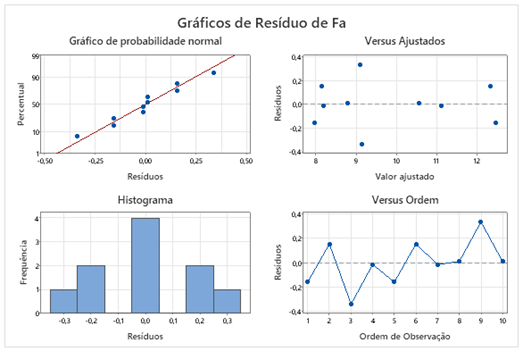
\includegraphics[width=0.8\linewidth]{Imagens/residuo 1.png}
    \smallcaption{Fonte: Autor}
    \label{fig:res1}
\end{figure}

Ao examinar os Gráficos \ref{fig:res1}, tem-se a capacidade de julgar a eficácia da análise realizada, ou seja, determinar se os resultados são verossímeis ou não. Essa avaliação é conduzida da seguinte maneira:

•	Gráfico de Probabilidade Normal: Uma análise de alta qualidade é indicada quando os pontos seguem a trajetória da linha vermelha. Neste caso, observamos que essa conformidade está presente, sugerindo, portanto, uma análise confiável (Verossímil).

•	Versus Ajustado: Para ser considerada uma análise confiável, os pontos devem ser dispostos de maneira randômica e distantes entre si, sinalizando que o experimento foi conduzido de forma imparcial, sem influências negativas. Neste cenário, essa disposição está um pouco distinta da ideal, podendo ter seus pontos ainda mais distantes e randômicos, caracterizando uma análise boa, mas não ideal (Verossímil em partes).

•	Histograma: A expectativa é que se assemelhe o máximo possível a uma curva de distribuição normal. Existe tal conformidade nesta análise indicada, sugerindo, portanto, uma análise confiável (Verossímil).

•	Versus Ordem: Para ser considerada uma análise sólida, o gráfico deve estar desordenado e com ausência de padrões aparentes. No caso analisado, essa particularidade não está completamente presente, afinal, observando o gráfico pode-se notar um certo padrão, indicando dessa forma, que a análise não é ideal (Não inteiramente verossímil).

\subsection{Regressão Fatorial (Momento torsor em função de fn, Vc, Refrigeração)} \label{regressão mt}

\begin{table}[!htb]
 \centering
    \caption{Análise de Variância (Mt)}
    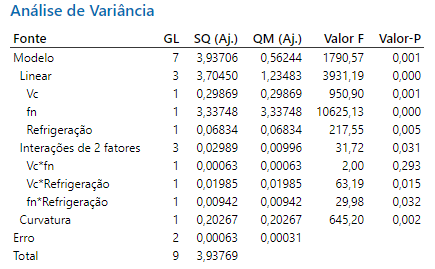
\includegraphics[width=0.8\linewidth]{Imagens/variancia 2.png}
    \smallcaption{Fonte: Autor}
    \label{tab:var2}
 \end{table}

Realizar-se-á agora uma análise semelhante a feita na tabela \ref{tab:var1}, fornecendo novamente uma variedade de informações valiosas, que auxiliarão na indicação de quais dos parâmetros utilizados (fn, Vc e refrigeração), mais influenciam no momento torsor.

Ao examinar a coluna "Valor P", destaca-se que os valores associados ao avanço (fn) são os menores da tabela, porém nota-se também, que os outros parâmetros analisados (Vc e Refrigeração) também estão abaixo de 0,05 (valor de alpha). Essa constatação aponta para uma confiança substancial, de aproximadamente 95\%, indicando que o avanço (fn) é a variável que mais influência no momento torsor, mas que as outras duas variáveis também exercem uma influência notável no esforço de momento torsor.

Ao focar na mesma tabela, mas agora na coluna "Valor F", torna-se notável que o avanço (fn) apresenta novamente o maior Valor F. Esse resultado sugere que a curva associada a esse parâmetro, a ser discutida nos próximos tópicos, terá uma inclinação considerável.

Porém, nota-se também que os outros dois parâmetros (Vc e refrigeração), também contam com valores relativamente altos na tabela de Valor F, indicando que mesmo que menor, também terão uma inclinação considerável nas respectivas curvas associadas a estes parâmetros, que serão discutidas nos próximos tópicos.
Portanto, podemos inferir que o avanço desempenha o papel mais significativo no esforço analisado (Momento torsor), mas que a Velocidade de corte e a Refrigeração, também tem uma influência relativamente considerável no esforço analisado.

\begin{figure}[!htp]
    \centering
    \caption{Gráfico de Pareto dos Efeitos Padronizados (Mt)}
    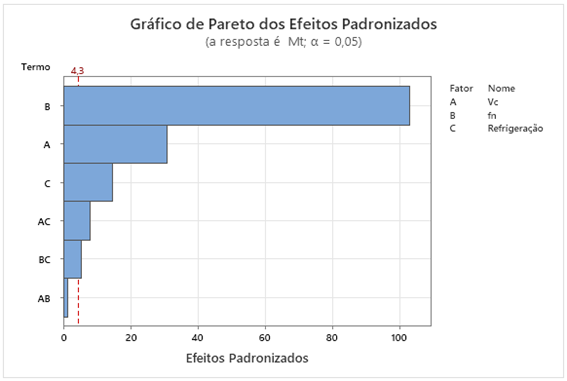
\includegraphics[width=0.8\linewidth]{Imagens/pareta 2.png}
    \smallcaption{Fonte: Autor}
    \label{fig:par2}
\end{figure}

Através do Gráfico \ref{fig:par2}, pode-se confirmar o resultado da análise realizada na tabela 5, tornando-se perceptível que o parâmetro de avanço exerce a maior influência no momento torsor, mas que os outros parâmetros (Velocidade de corte (Vc) e Refrigeração) também influenciam com certa relevância no momento torsor. Essa constatação é respaldada pelo fato de todas estas variáveis estarem posicionadas à direita da linha vermelha evidenciada no gráfico. Em outras palavras, valores à direita dessa linha exercem uma influência mais marcante no momento torsor. 

Vale analisar também, que a combinação entre velocidade de corte e refrigeração, e a combinação entre avanço e refrigeração, também exercem uma certa influência no momento torsor, mesmo que de forma menos significativa do que os outros parâmetros. Isso porque estas combinações também ultrapassam para o lado direito da linha vermelha.

Cabe ressaltar que esses resultados foram obtidos considerando um Alpha de 0,05, conferindo uma confiança de 95\%. 

 \begin{figure}[!htp]
    \centering
    \caption{Gráficos de resíduo de Mt}
    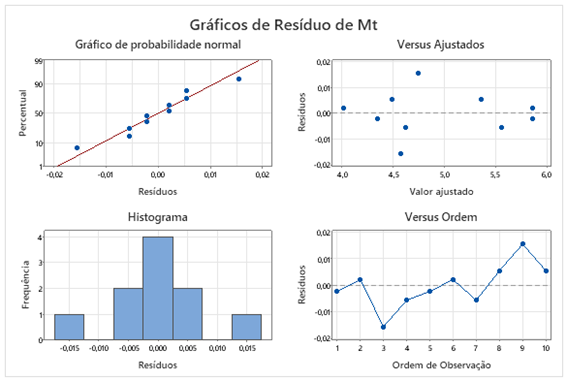
\includegraphics[width=0.8\linewidth]{Imagens/residuo 2.png}
    \smallcaption{Fonte: Autor}
    \label{fig:res2}
\end{figure}

Será feito agora uma análise semelhante a realizada para o gráfico \ref{fig:res1}, porém agora com o objetivo de julgar a eficácia da análise de momento torsor realizada, ou seja, determinar se os resultados são verossímeis ou não. Essa avaliação é conduzida da seguinte maneira:

•	Gráfico de Probabilidade Normal: Uma análise de alta qualidade é indicada quando os pontos seguem a trajetória da linha vermelha. Neste caso, observamos que essa conformidade está presente, apesar de alguns pontos estarem levemente fora da linha, sugerindo, portanto, uma análise de certa forma confiável (Verossímil).

•	Versus Ajustado: Para ser considerada uma análise confiável, os pontos devem ser dispostos de maneira randômica e distantes entre si, sinalizando que o experimento foi conduzido de forma imparcial, sem influências negativas. Neste cenário, assim como o do gráfico 2 essa disposição está um pouco distinta da ideal, podendo ter seus pontos ainda mais distantes e randômicos, caracterizando uma análise boa, mas não ideal (Verossímil em partes).

•	Histograma: A expectativa é que se assemelhe o máximo possível a uma curva de distribuição normal. Novamente, assim como no gráfico 2, existe tal conformidade nesta análise indicada, sugerindo, portanto, uma análise confiável (Verossímil).

•	Versus Ordem: Para ser considerada uma análise sólida, o gráfico deve estar desordenado e com ausência de padrões aparentes. No caso analisado, pode-se notar um pequeno padrão em seus pontos, tratando-se portanto de uma analise boa, mas não ideal (razoavelmente verossímil).

\section{Factorial Plots}

A etapa subsequente de análise, realizada durante o estudo dos esforços, valida os resultados obtidos anteriormente no tópico \ref{regressao}, empregando métodos diversos.

\subsection{Gráficos fatoriais (Força de avanço)}

 \begin{figure}[!htp]
    \centering
    \caption{Gráfico de efeitos principais para Fa}
    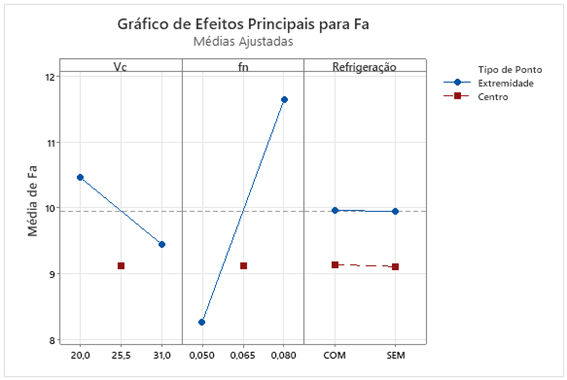
\includegraphics[width=0.8\linewidth]{Imagens/efeitos1.png}
    \smallcaption{Fonte: Autor}
    \label{fig:efe1}
\end{figure}

Mediante a observação do Gráfico \ref{fig:efe1}, é possível validar e confirmar a análise realizada no tópico \ref{regressaof}, demonstrado qual dos três parâmetros utilizados (avanço, velocidade de corte e refrigeração) exerce a influência mais direta sobre a força de avanço. 

Torna-se evidente que a curva mais acentuada (com o maior grau de inclinação) corresponde ao avanço (fn) revelando e confirmando que este é o parâmetro que exerce a maior e mais direta influência sobre a força de avanço.

 \begin{figure}[!htp]
    \centering
    \caption{Gráfico de interação para Fa}
    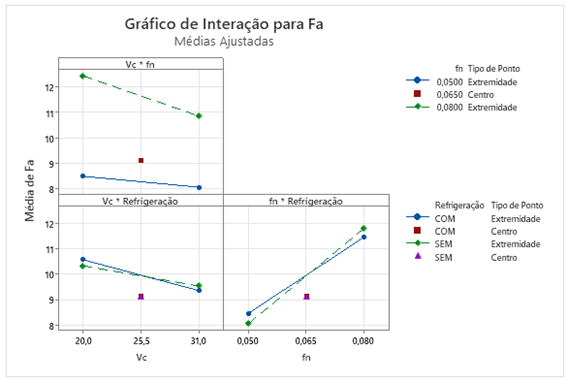
\includegraphics[width=0.8\linewidth]{Imagens/interação1.png}
    \smallcaption{Fonte: Autor}
    \label{fig:int1}
\end{figure}

O Gráfico \ref{fig:int1} oferece uma perspectiva única em comparação às análises anteriores, uma vez que relaciona dois parâmetros distintos em uma única representação gráfica, evidenciando como a interação entre esses dois parâmetros afeta a força de avanço.
 
Por meio desse gráfico, percebe-se que a maior inclinação é observada ao combinar o avanço (fn) com a refrigeração, sugerindo que essa conjunção de parâmetros exerce a influência mais pronunciada na força de avanço.

\newpage
\subsection{Gráficos fatoriais (momento torsor)}

 \begin{figure}[!htp]
    \centering
    \caption{Gráfico de efeitos principais para Mt}
    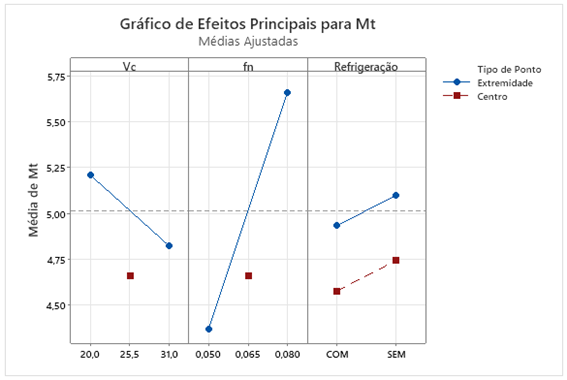
\includegraphics[width=0.8\linewidth]{Imagens/efeitos2.png}
    \smallcaption{Fonte: Autor}
    \label{fig:efe2}
\end{figure}

Por meio da análise do Gráfico \ref{fig:efe2}, é possível validar e ratificar a avaliação realizada no segmento \ref{regressão mt}, esclarecendo qual dos três parâmetros considerados (avanço, velocidade de corte e refrigeração) tem a maior influência sobre o momento torsor. 

Fica evidente que a curva mais pronunciada (com a maior inclinação) pertence ao avanço (fn), confirmando que este é o parâmetro que exerce a maior e mais proeminente influência sobre a força de avanço. Porém, assim como indicavam as análises de Valor F da tabela \ref{tab:var2}, os parâmetros de velocidade de corte e refrigeração, também contam com uma certa inclinação, indicando e confirmando assim que, segundo a análise desenvolvida, estes parâmetros também tem uma influência razoável no momento torsor.

\begin{figure}[!htp]
    \centering
    \caption{Gráfico de interação para Mt}
    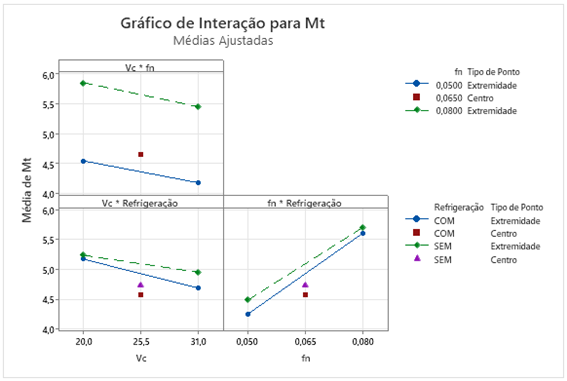
\includegraphics[width=0.8\linewidth]{Imagens/interação2.png}
    \smallcaption{Fonte: Autor}
    \label{fig:int2}
\end{figure}

O Gráfico \ref{fig:int2}, proporciona uma perspectiva singular se comparado às análises anteriores, pois novamente uni dois parâmetros distintos em uma única representação gráfica, revelando como a interação entre esses fatores impacta no esforço analisado, que neste caso é o momento torsor. 

Ao examinar essa representação gráfica, é perceptível que, assim como para a força de corte, a inclinação mais pronunciada é alcançada ao associar o avanço (fn) à refrigeração. Indicando que essa combinação de parâmetros exerce a influência mais expressiva no momento torsor. 


\chapter{Conclusões}

Conclui-se, portanto, que em decorrência da análise dos esforços de furação no torno, torna-se inegável que o avanço emerge como a variável de maior impacto sobre ambos os esforços estudados (força de avanço e o momento torsor). Mas que ao explorar mais profundamente o efeito sobre o momento torsor, outros parâmetros, como a velocidade de corte e a refrigeração da peça, também revelaram-se como influências significativas, mesmo que em menor quantidade se comparadas ao parâmetro de avanço. 

Em suma, a análise dos esforços de furação no torno apresentou resultados que, em sua maioria, demonstram uma acurácia satisfatória. Embora os dados obtidos não alcancem a perfeição absoluta, é crucial destacar que a margem de diferença observada está dentro de limites aceitáveis.

Durante o curso deste estudo, é importante reconhecer que certas imprecisões podem ter sido introduzidas durante a aquisição dos dados. Estas variações podem ser atribuídas a possíveis erros experimentais, tolerâncias de medição ou até mesmo a limitações intrínsecas aos métodos empregados. A compreensão destas potenciais fontes de discrepância é fundamental para interpretar os resultados de maneira crítica.

Apesar das nuances mencionadas, é encorajador observar que os objetivos finais delineados no início do relatório foram cumpridos com êxito. A análise dos esforços de furação forneceu insights valiosos que contribuíram significativamente para a melhor compreensão aprofundada dos esforços de furação no torno.


\printbibliography

\end{document}